\documentclass[11pt,a4paper]{article}

\usepackage[utf8]{inputenc}
\usepackage[T1]{fontenc}
% Castellano si la instalacion de LaTeX lo tiene (MacTeX completo, o
% texlive-lang-spanish en Linux); si no, el documento igual compila.
\IfFileExists{spanish.ldf}
  {\usepackage[spanish,es-nodecimaldot]{babel}}
  {\usepackage[english]{babel}\PackageWarningNoLine{informe}
   {babel-spanish no esta instalado: la separacion silabica no sera la correcta}}
\usepackage{amsmath,amssymb}
\usepackage{booktabs}
\usepackage{graphicx}
\usepackage{caption}
\usepackage{geometry}
\usepackage{natbib}
\usepackage[hidelinks]{hyperref}

\geometry{margin=2.5cm}
% Margen de maniobra para que TeX afloje el espaciado en vez de desbordar
% el margen en parrafos con nombres de variables largos en \texttt{}.
\emergencystretch=2em
\bibliographystyle{plainnat}
\setcitestyle{authoryear,round}
\graphicspath{{../output/figures/}}

% Parametros estimados, generados por los programas de programs/.
% Si estos archivos no existen, correr 02_descriptivas.py y 03_modelos.py.
% Generado por 03_modelos.py. No editar a mano.
\newcommand{\plalpha}{2.92}
\newcommand{\plxmin}{22}
\newcommand{\nPanel}{114{,}714}
\newcommand{\nTrain}{80{,}299}
\newcommand{\nTest}{34{,}415}
\newcommand{\umbralHit}{70}
\newcommand{\tasaBase}{1.03}
\newcommand{\nHitsTest}{353}
\newcommand{\nPosPL}{408}
\newcommand{\nPosRF}{375}
\newcommand{\nObjetivo}{354}

% Cociente de verosimilitud normalizado power law vs lognormal
% R = -83.6732, p = 0.0000
\newcommand{\plR}{-83.67}
\newcommand{\plp}{< 0.001}


\title{\textbf{¿Cómo predecir un súper hit?}\\[.3em]
       \large Un análisis comparativo de modelos de popularidad musical}
\author{Catalina Gallardo \and Manuel Elorga}
\date{E337: Big Data --- Universidad de San Andrés}

\begin{document}
\maketitle

\begin{abstract}
\noindent
La popularidad musical en plataformas de streaming está extremadamente
concentrada: una fracción mínima de canciones acumula la mayor parte de la
atención. Este trabajo compara dos maneras de identificar a esas canciones
excepcionales ---las que llegan al 1\% más popular--- usando un panel de
\nPanel{} canciones observadas en 2018 y 2019. La primera aprovecha
únicamente la estructura estadística de la distribución de popularidad,
ajustando una ley de potencia por máxima verosimilitud sobre la popularidad
del año anterior. La segunda es un Random Forest que utiliza exclusivamente
los atributos acústicos de cada canción. El contraste es nítido: la
popularidad pasada identifica a los súper hits con un AUC cercano a uno,
mientras que los atributos acústicos, aunque ordenan a las canciones bastante
mejor que el azar, quedan muy por detrás y recuperan apenas una fracción
mínima de los súper hits. El éxito
extremo resulta ser muy persistente en el tiempo, pero no se deja explicar
por las características sonoras de la canción.
\end{abstract}

\section{Introducción}

La industria musical se transformó con la llegada de las plataformas
digitales de streaming. Spotify, que concentra una porción dominante del
mercado, publica para cada canción un \textit{popularity score} entre 0 y
100. La distribución de ese score está lejos de ser simétrica: la mayoría de
las canciones se agrupa en valores bajos, mientras unas pocas alcanzan
niveles muy altos. Esa asimetría no es un detalle estadístico sino el rasgo
central del mercado, y es lo que vuelve interesante la pregunta por el éxito
extremo.

De ahí surge una pregunta con consecuencias prácticas para artistas, sellos y
plataformas: \textbf{¿se puede anticipar cuáles canciones van a alcanzar el
éxito extremo?} Y, sobre todo, ¿con qué información? Hay dos respuestas
posibles, conceptualmente muy distintas:

\begin{enumerate}
  \item \textbf{La estructura del mercado.} Si la popularidad se distribuye
        con una cola pesada, la propia forma de la distribución indica cuán
        probable es superar un umbral alto. Esta vía no mira a la canción:
        mira al mercado en el que compite.
  \item \textbf{Los atributos de la canción.} Si el éxito depende de
        cualidades sonoras ---qué tan bailable, enérgica o acústica es---
        entonces debería poder predecirse a partir de esos atributos. Es el
        enfoque dominante en la literatura, que reporta buenos desempeños con
        algoritmos de clasificación
        \citep{pareek2022,saragih2023,dimolitsas2023}.
\end{enumerate}

Este trabajo pone las dos a competir sobre los mismos datos y con la misma
regla de evaluación. La pregunta que organiza el análisis es cuánta de la
estructura de cola que exhibe la popularidad logra recuperar un modelo de
aprendizaje automático que solo observa atributos acústicos.

\section{Datos}

\subsection{Fuente y construcción}

Partimos de dos bases publicadas en Kaggle \citep{kaggle_spotify} con el
score de popularidad y los atributos acústicos de canciones de Spotify,
medidos en 2018 y en 2019. Las bases fueron construidas con el endpoint de
\textit{audio features} de la API de Spotify, que desde entonces fue
discontinuado; esto hace que los datos no sean reproducibles hoy desde la
fuente original, y es una de las razones por las que el repositorio conserva
los archivos crudos.

Para enriquecer el análisis consultamos la API de Spotify y agregamos, para
cada canción, metadata de álbum y de artista: fecha de publicación, tipo de
álbum, número de pista, si la canción es explícita y la cantidad de artistas
acreditados. A partir de la fecha de publicación construimos la edad de la
canción.

\subsection{Limpieza}

Eliminamos canciones duplicadas por identificador, descartamos las que no
tienen fecha de publicación recuperable ---típicamente porque fueron dadas de
baja de la plataforma--- y excluimos aquellas cuya fecha de publicación es
posterior al año de medición, que corresponden a reediciones o versiones y
tendrían una edad negativa.

El análisis se realiza sobre el panel de canciones presentes en ambos años,
que permite observar la misma canción en dos momentos. Quedan \nPanel{}
canciones.

\subsection{Descripción}

\begin{table}[htbp]
\caption{Estadística descriptiva del score de popularidad de Spotify.}
\label{tab:descriptivas}
\begin{tabular}{rrrrrrr}
\toprule
Año & N & Media & Desvío & p50 & p99 & Max \\
\midrule
2018 & 115373 & 24.25 & 17.90 & 22.00 & 70.00 & 100 \\
2019 & 129436 & 24.17 & 19.67 & 22.00 & 72.00 & 100 \\
\bottomrule
\end{tabular}
\end{table}


La Tabla~\ref{tab:descriptivas} muestra el rasgo que motiva el trabajo. La
popularidad media ronda los 24 puntos sobre 100 y la mediana está en 22, pero
el percentil 99 se ubica en 70 y el máximo alcanza el tope de la escala. La
distribución es estable entre años en sus momentos centrales, de modo que lo
que cambia no es el nivel general de popularidad sino qué canciones ocupan el
extremo.

\begin{table}[htbp]
\caption{Canciones más populares de cada año (score entre paréntesis).}
\label{tab:top}
\begin{tabular}{p{.45\textwidth}p{.45\textwidth}}
\toprule
2018 & 2019 \\
\midrule
thank u, next --- Ariana Grande (100) & Con Calma --- Daddy Yankee (100) \\
Taki Taki (with Selena Gomez, Ozuna \& Cardi B) --- DJ Snake (99) & Wow. --- Post Malone (98) \\
MIA (feat. Drake) --- Bad Bunny (97) & Sucker --- Jonas Brothers (98) \\
\bottomrule
\end{tabular}
\end{table}


\begin{figure}[htbp]
  \centering
  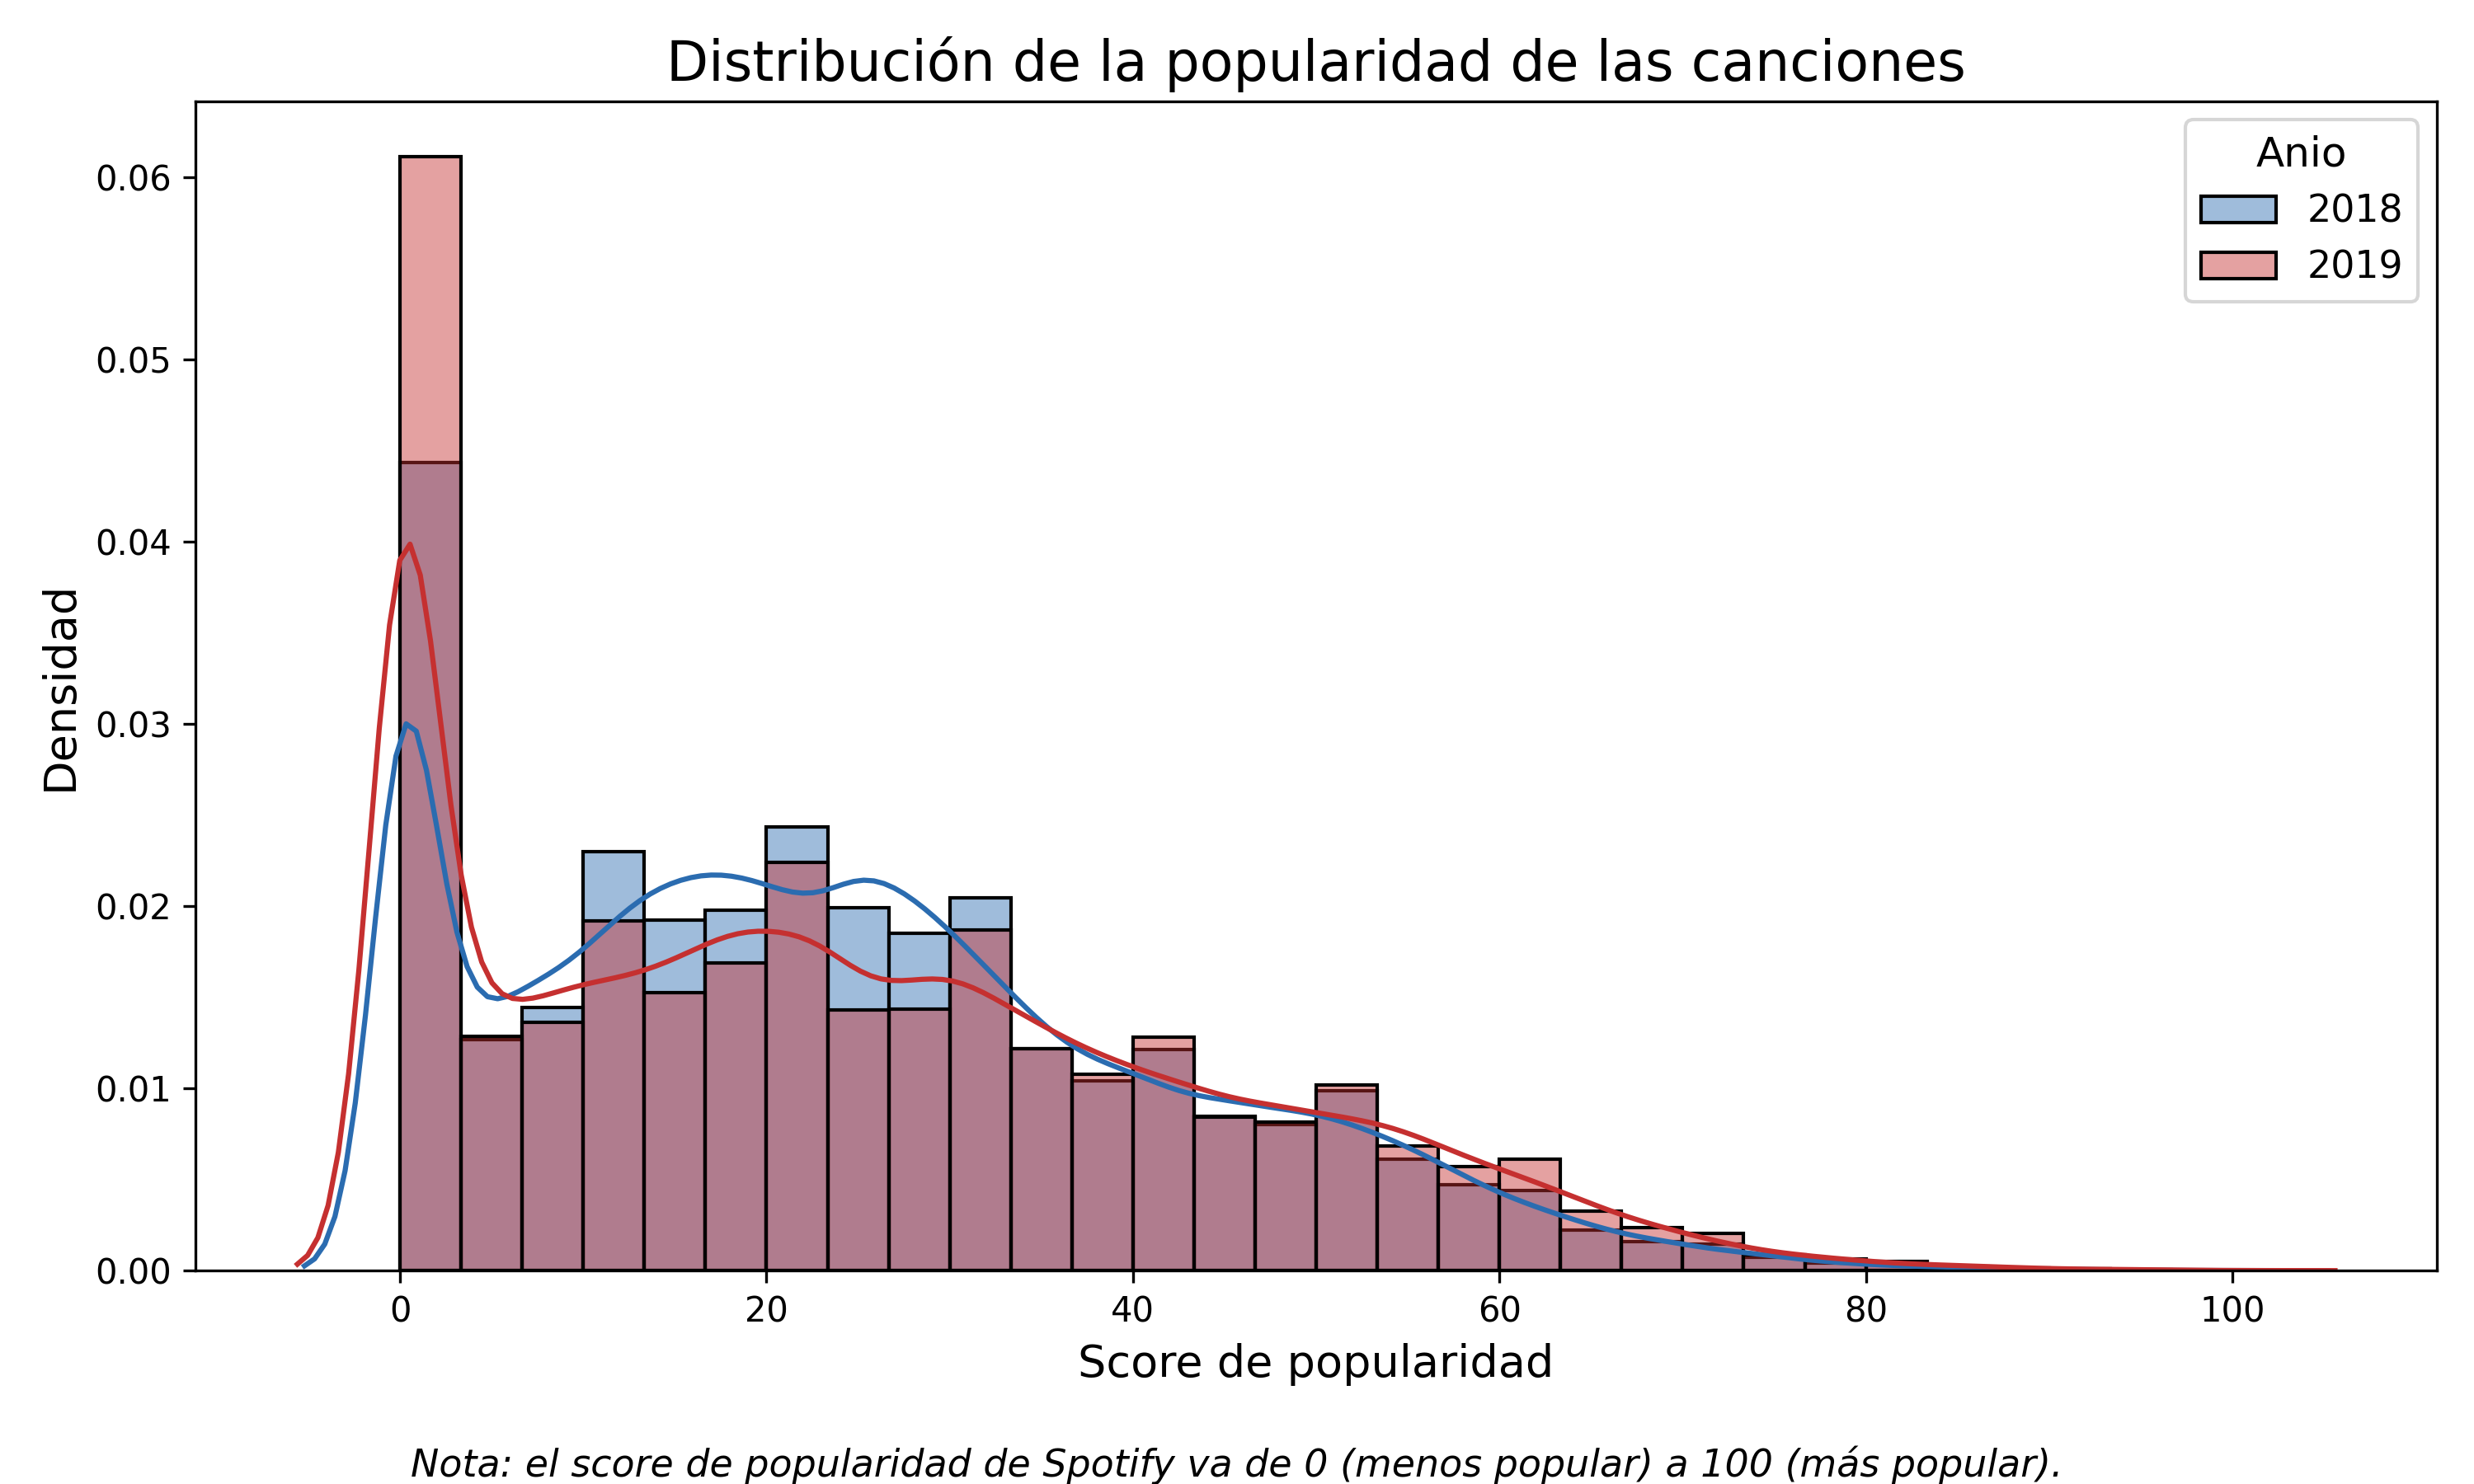
\includegraphics[width=.85\textwidth]{popularidad.png}
  \caption{Distribución del score de popularidad en 2018 y 2019. Las dos
           distribuciones son casi indistinguibles y marcadamente asimétricas
           a la derecha.}
  \label{fig:popularidad}
\end{figure}

\section{Metodología}

\subsection{Definición de súper hit}

Definimos como súper hit a toda canción que en 2019 se ubica en el percentil
99 o más alto de popularidad, lo que corresponde a un score de \umbralHit{}
puntos o más. Bajo esta definición, \tasaBase\% de las canciones del panel
son súper hits. El fuerte desbalance de clases no es un inconveniente del
diseño: es exactamente el fenómeno que se quiere estudiar.

\subsection{Modelo 1: ley de potencia estimada por máxima verosimilitud}

Una variable sigue una ley de potencia si su densidad decae como
$p(x) \propto x^{-\alpha}$ por encima de un umbral $x_{\min}$. La función de
supervivencia correspondiente, es decir la probabilidad de superar un valor
dado, es
\begin{equation}
  P(X \geq x) \;=\; \left(\frac{x}{x_{\min}}\right)^{1-\alpha},
  \qquad x \geq x_{\min}.
  \label{eq:supervivencia}
\end{equation}

Estimamos $\alpha$ y $x_{\min}$ por máxima verosimilitud siguiendo el
procedimiento de \citet{clauset2009}, implementado en el paquete
\texttt{powerlaw} \citep{alstott2014}. La estimación por máxima verosimilitud
es preferible a una regresión log-log sobre el histograma, que produce
estimadores sesgados en colas pesadas.

El ajuste se realiza sobre la popularidad de 2018 en la muestra de
entrenamiento y arroja $\hat{\alpha} = \plalpha$ y
$\hat{x}_{\min} = \plxmin$. Para cada canción de la muestra de testeo
evaluamos la ecuación~\eqref{eq:supervivencia} en su popularidad de
\textbf{2018} y usamos $1 - P(X \geq x)$ como puntaje: el percentil estimado
que la canción ocupa en la distribución. Para valores por debajo de
$x_{\min}$ la ley no está definida ---el ajuste describe solo la cola--- y el
puntaje se fija en cero.

Conviene subrayar que este modelo utiliza la popularidad del año anterior y
no la del año que se predice. Así, la predicción es genuinamente fuera de
muestra en el tiempo, y la comparación con el Random Forest es una
comparación entre dos conjuntos de información distintos: la trayectoria
previa de la canción frente a sus cualidades sonoras.

\subsection{Modelo 2: Random Forest sobre atributos acústicos}

El segundo modelo es un Random Forest \citep{breiman2001}, el algoritmo que
la literatura revisada señala como el de mejor desempeño para esta tarea.
Utiliza trece atributos acústicos provistos por Spotify
---\textit{acousticness}, \textit{danceability}, duración, \textit{energy},
\textit{instrumentalness}, \textit{key}, \textit{liveness},
\textit{loudness}, \textit{mode}, \textit{speechiness}, \textit{tempo},
\textit{time signature} y \textit{valence}--- más la cantidad de artistas
acreditados, un indicador de contenido explícito y la edad de la canción.
Deliberadamente no incluye la popularidad pasada, de modo que su conjunto de
información sea el de los atributos de la canción.

Los hiperparámetros se eligen por validación cruzada estratificada de cinco
pliegues sobre la muestra de entrenamiento \citep{james2021}, maximizando el
AUC. Elegir en
función del AUC y no de la proporción de aciertos es necesario con una clase
positiva del 1\%: una regla que nunca predice un hit ya alcanza un 99\% de
aciertos, de manera que la proporción de aciertos no distingue entre
candidatos.

\subsection{Regla de decisión y evaluación}

Dividimos el panel en entrenamiento (70\%) y testeo (30\%) de forma
estratificada, con \nTrain{} y \nTest{} canciones respectivamente. Todas las
métricas que se reportan corresponden a la muestra de testeo.

Por el mismo desbalance, clasificar como positivo todo caso con probabilidad
estimada mayor a $0.5$ no es informativo: casi ningún caso supera ese valor y
precisión y sensibilidad colapsan a cero para ambos modelos. Calibramos
entonces el umbral de cada modelo de modo que clasifique como positiva
aproximadamente la misma proporción de casos que la tasa base, lo que sobre la
muestra de testeo equivale a \nObjetivo{} predicciones positivas.

La calibración no puede ser exacta, porque ninguno de los dos puntajes es
continuo y se producen empates en el valor de corte. El caso de la ley de
potencia es el más marcado: la popularidad es una variable entera y el puntaje
es una función de ella, de modo que toma pocos valores distintos y todas las
canciones con la misma popularidad de 2018 reciben el mismo puntaje, y entran o
salen juntas. El Random Forest tiene el mismo problema en menor medida, porque
su probabilidad estimada es la proporción de árboles que votan por la clase
positiva y sólo puede tomar múltiplos de uno sobre el número de árboles. La ley
de potencia emite así \nPosPL{} predicciones positivas y el Random Forest
\nPosRF{}, frente a las \nObjetivo{} que marcaría la tasa base y a
\nHitsTest{} súper hits efectivos en la muestra de testeo. Las matrices de confusión son comparables
con esa salvedad, que juega en contra de la ley de potencia: al emitir más
predicciones positivas, su precisión se calcula sobre una base más exigente. El
AUC, que no depende del umbral elegido, no está afectado por este problema y se
reporta como medida global de capacidad de discriminación.

\section{Resultados}

\subsection{¿Es realmente una ley de potencia?}

Antes de usar la ley de potencia conviene preguntarse si describe bien a los
datos. La Figura~\ref{fig:ajuste} compara la función de supervivencia
empírica con la ley de potencia ajustada y con una lognormal. El test de
cociente de verosimilitudes normalizado entre ambas alternativas arroja
$R = \plR$ con $p \plp$, lo que favorece a la lognormal de manera
estadísticamente significativa.

\begin{figure}[htbp]
  \centering
  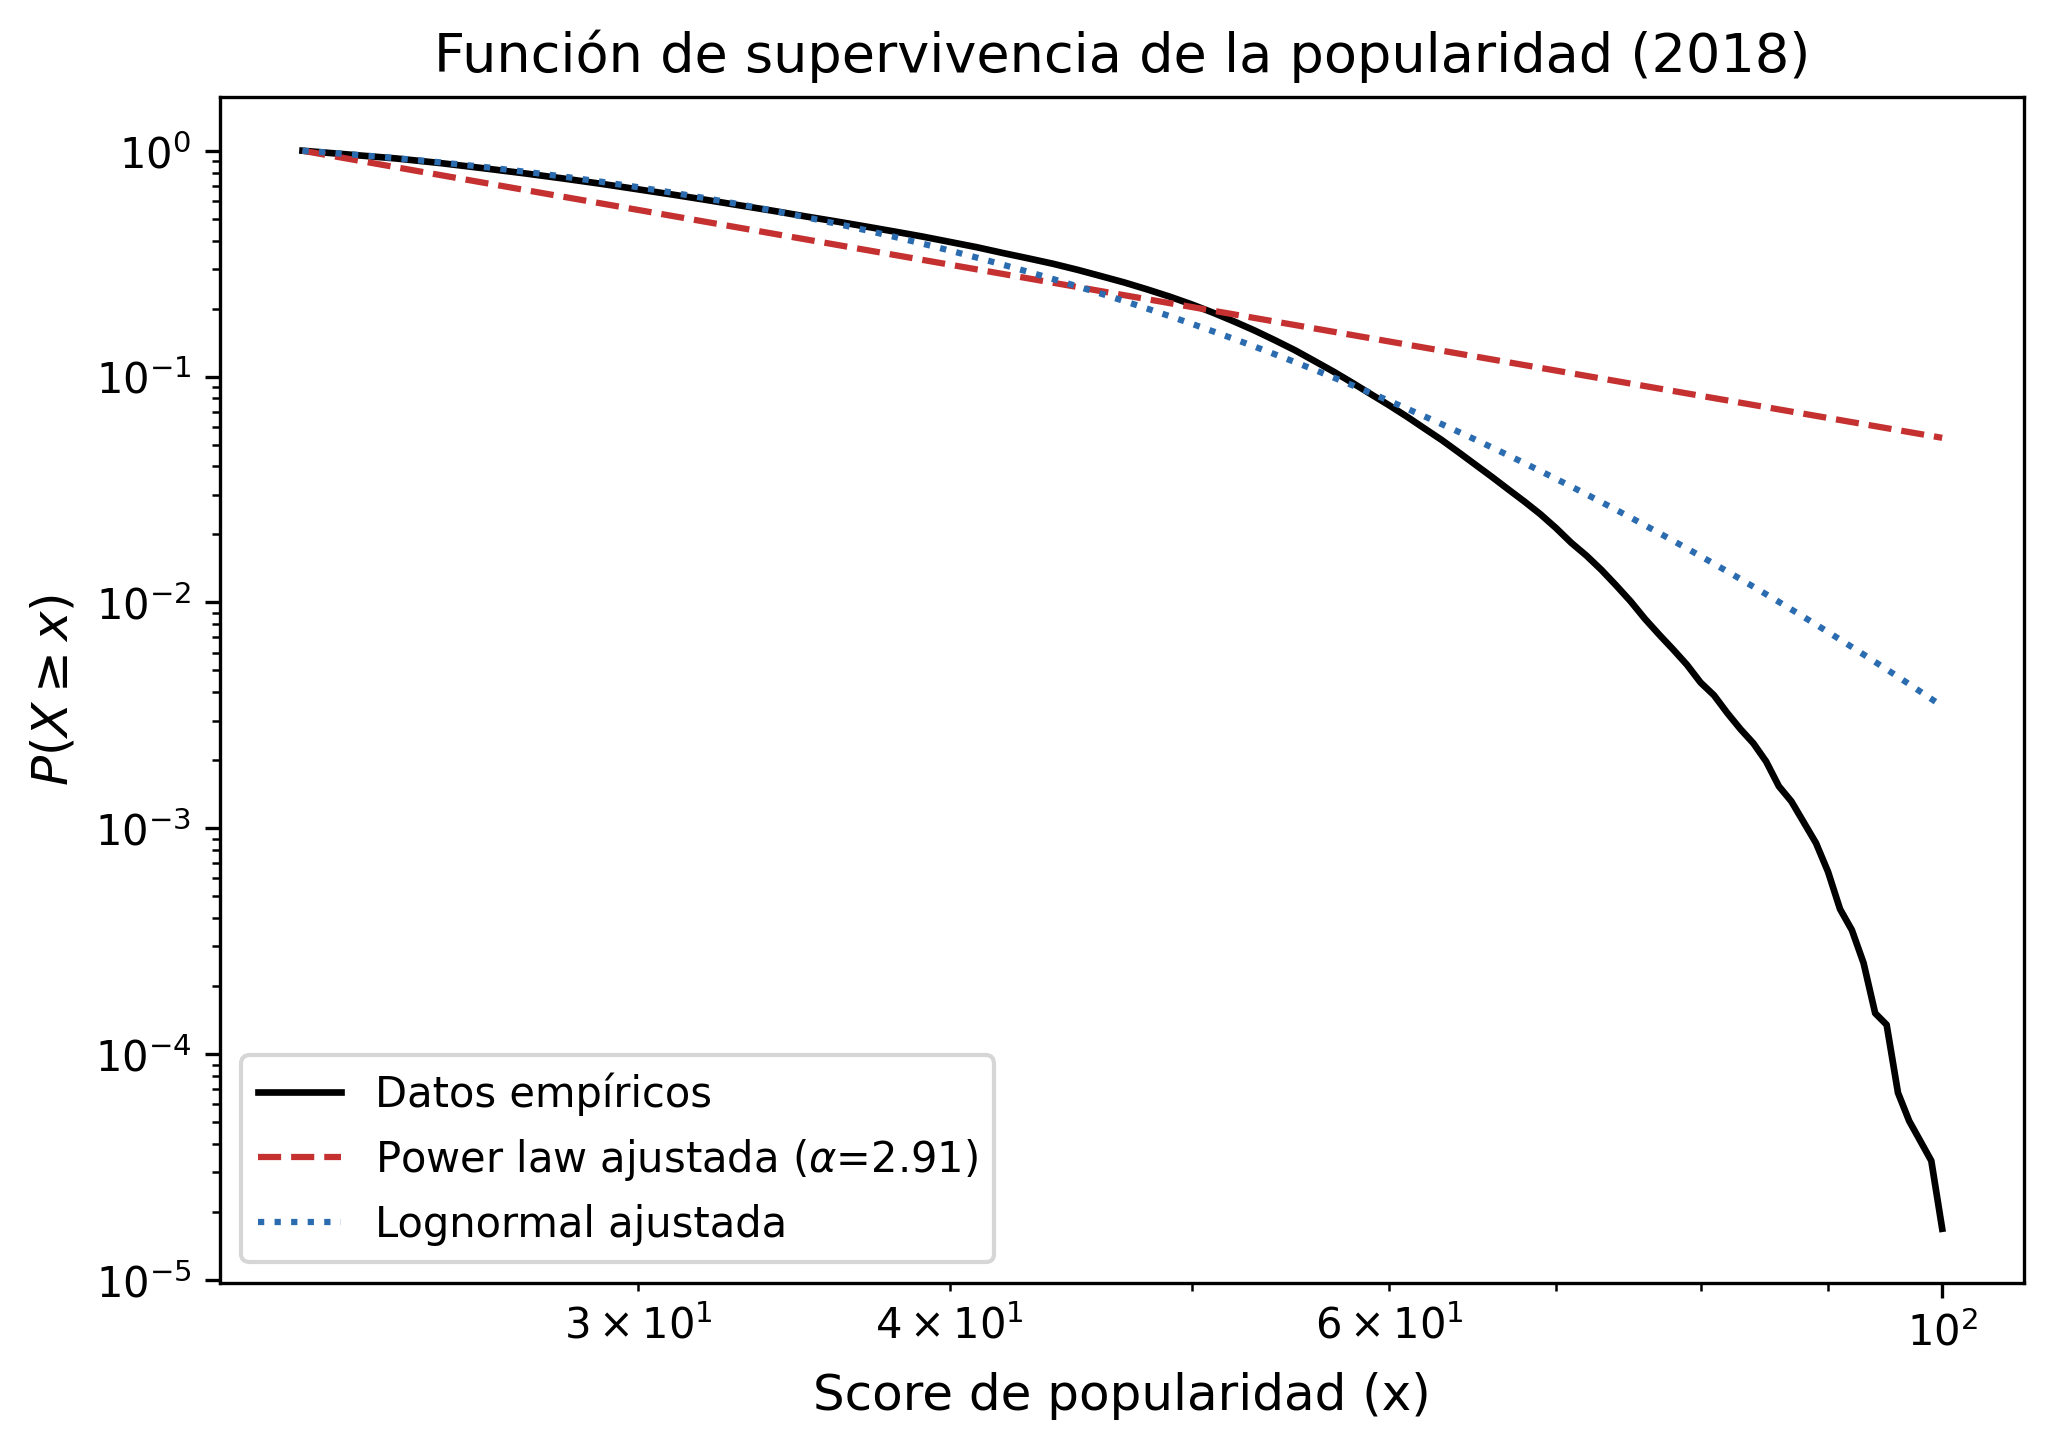
\includegraphics[width=.72\textwidth]{power-law-ajuste.png}
  \caption{Función de supervivencia de la popularidad en 2018, en escala
           logarítmica, junto con los ajustes de una ley de potencia y de una
           lognormal.}
  \label{fig:ajuste}
\end{figure}

Conviene entonces ser preciso sobre lo que se puede afirmar. La popularidad
tiene una cola derecha pesada, y ese hecho es robusto. Pero la ley de
potencia no es la mejor descripción paramétrica disponible, y además el score
está acotado entre 0 y 100, mientras que una ley de potencia genuina no tiene
cota superior. La ley de potencia funciona aquí como un resumen paramétrico
útil y parsimonioso de la cola, no como el proceso generador de los datos. Lo
que se evalúa a continuación es su desempeño como herramienta de
ordenamiento, que no depende de que el ajuste sea el mejor posible.

\subsection{Comparación de modelos}

\begin{table}[htbp]
\caption{Desempeño en la muestra de testeo para identificar canciones del top 1\% de popularidad en 2019. El umbral de clasificación de cada modelo se calibra a la tasa base de positivos.}
\label{tab:resultados}
\begin{tabular}{lrrrrr}
\toprule
Modelo & Accuracy & Precision & Recall & F1 & AUC \\
\midrule
Ley de potencia & 0.995 & 0.706 & 0.816 & 0.757 & 0.997 \\
Random Forest & 0.980 & 0.048 & 0.051 & 0.049 & 0.761 \\
RF + popularidad pasada & 0.995 & 0.744 & 0.748 & 0.746 & 0.986 \\
\bottomrule
\end{tabular}
\end{table}


La Tabla~\ref{tab:resultados} contiene el resultado central del trabajo, y la
diferencia es grande. La ley de potencia aplicada sobre la popularidad del
año anterior ordena a las canciones casi perfectamente: su AUC es
prácticamente uno y, con el umbral calibrado, acierta en torno a siete de
cada diez de sus predicciones positivas mientras recupera una amplia mayoría
de los súper hits efectivos. El Random Forest sobre atributos acústicos, en
cambio, queda muy por detrás. Su AUC es moderado ---claramente por encima del
azar, de modo que los atributos acústicos no son puro ruido--- pero la
distancia con la ley de potencia es enorme, y lo decisivo para la pregunta del
trabajo es que con el umbral calibrado recupera una fracción mínima de los
súper hits: tanto su precisión como su sensibilidad quedan por debajo del cinco
por ciento. Los atributos acústicos sirven para ordenar canciones, pero no para
identificar a las excepcionales.

\begin{figure}[htbp]
  \centering
  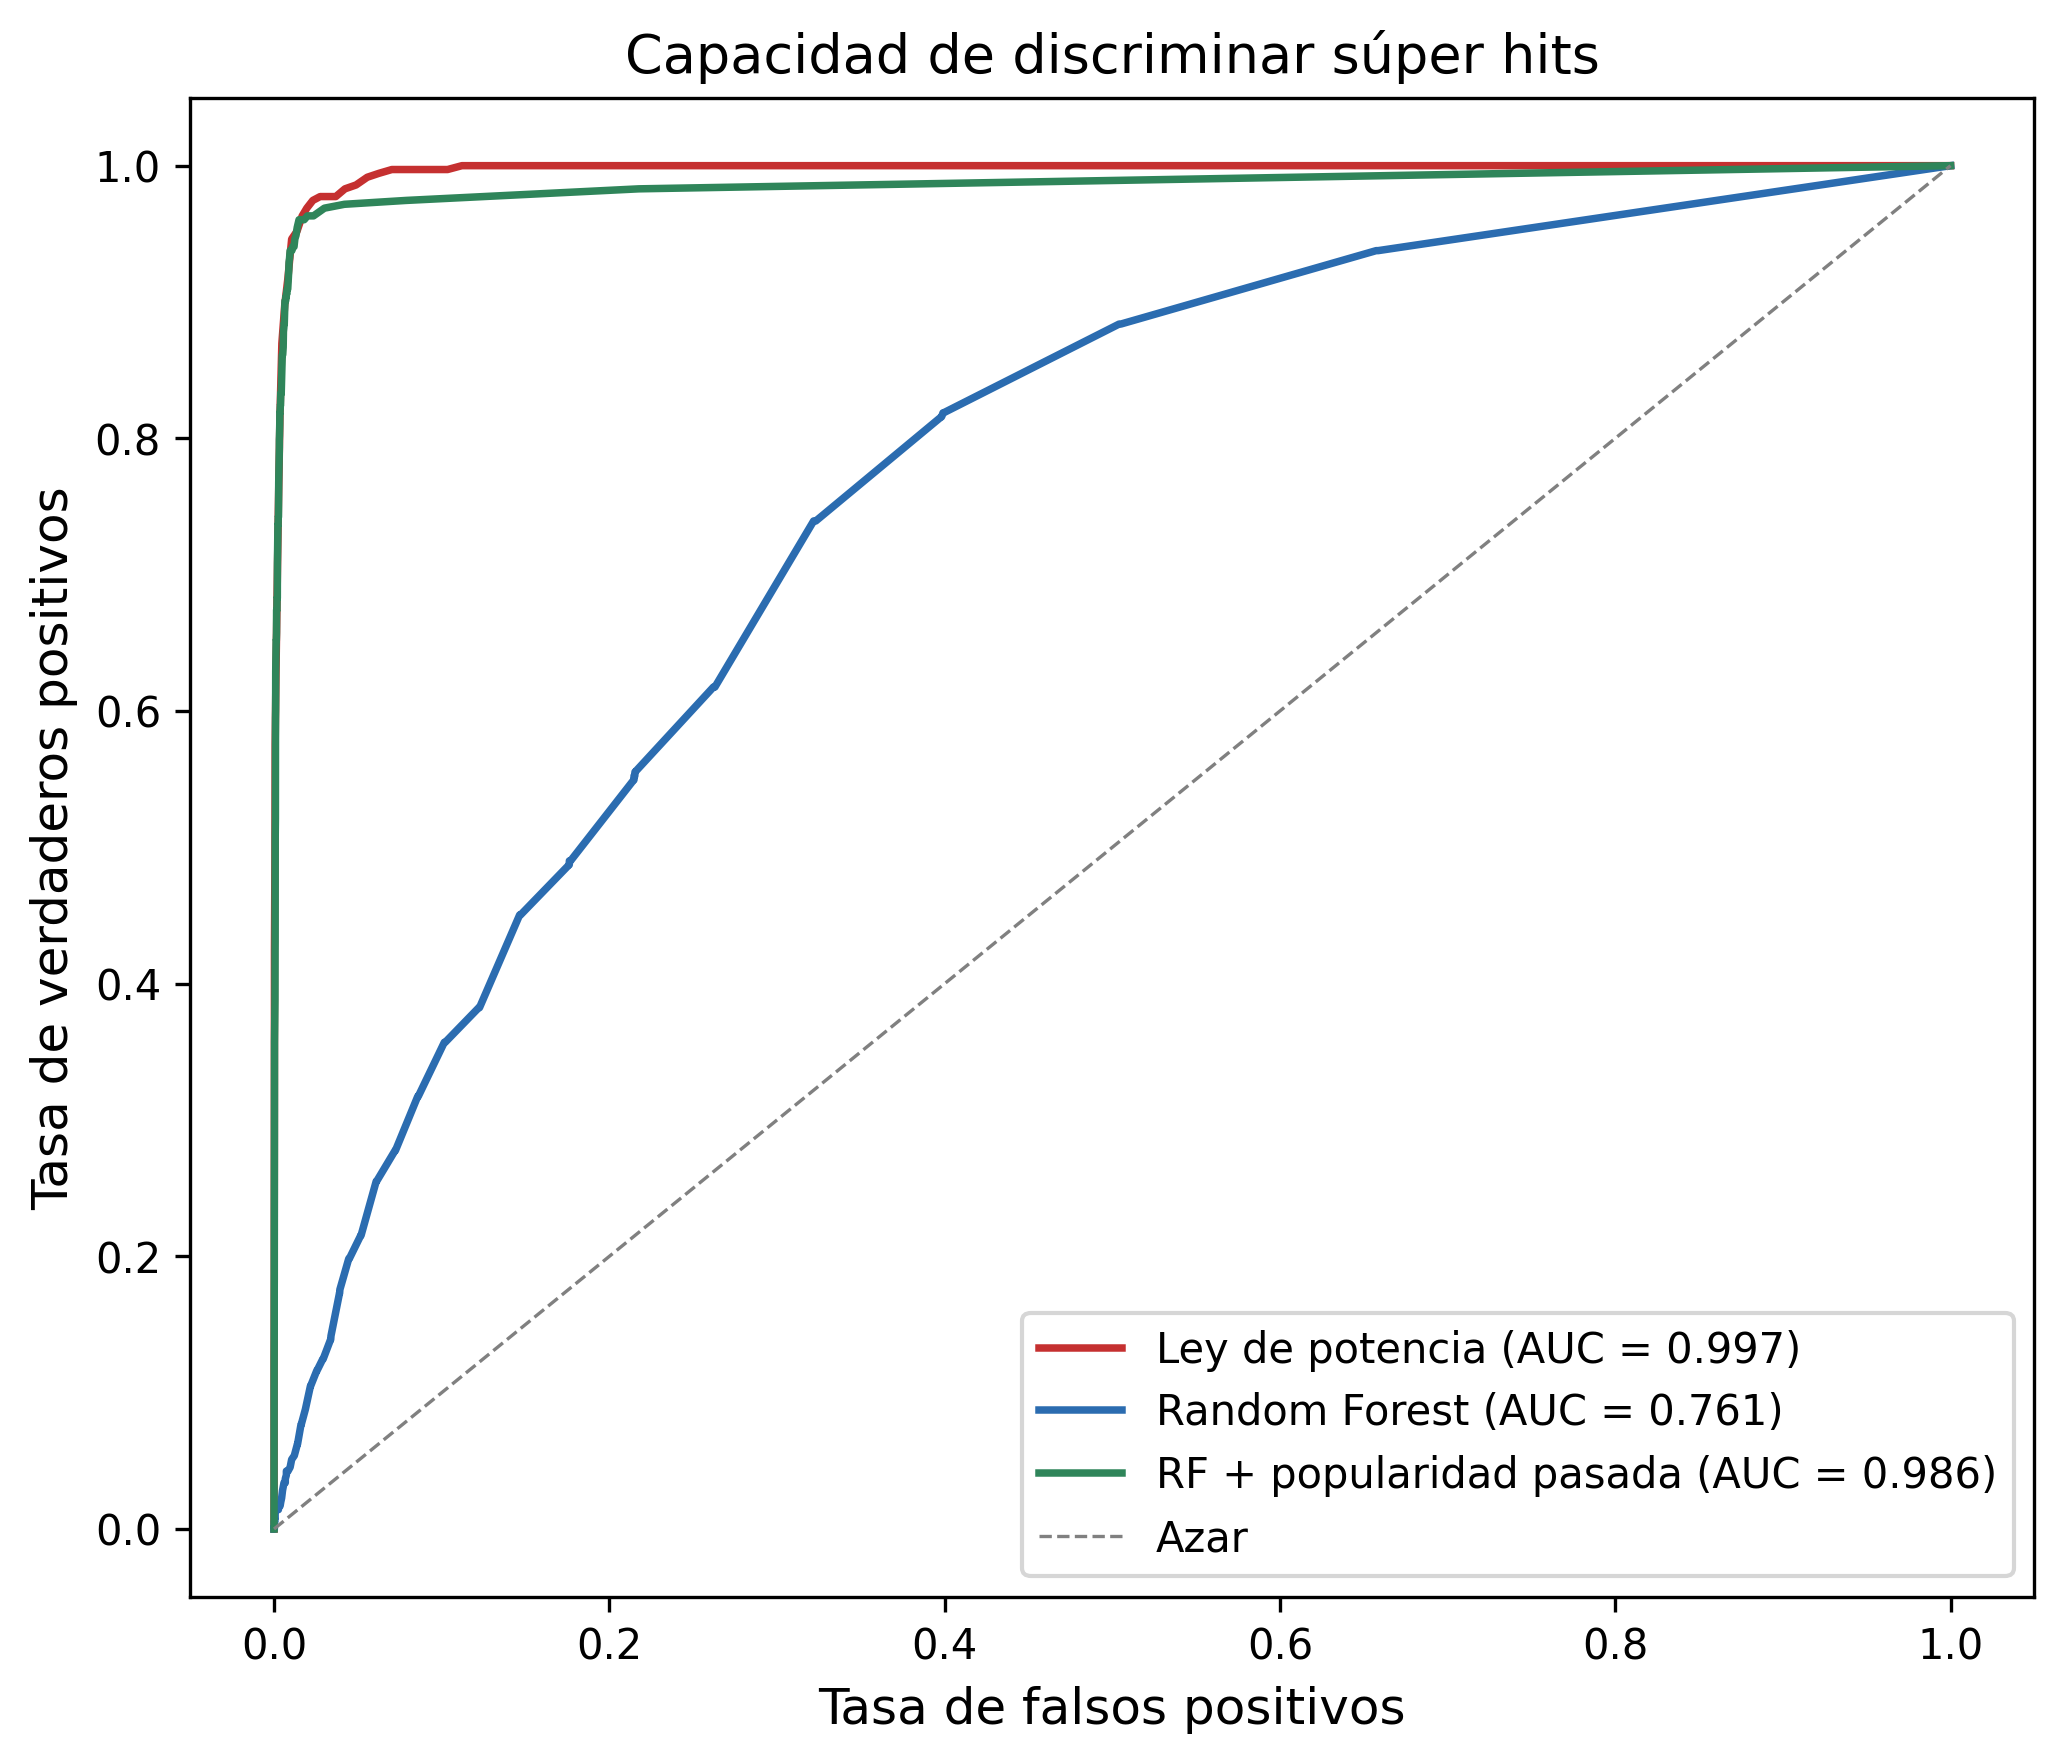
\includegraphics[width=.68\textwidth]{roc-comparacion.png}
  \caption{Curvas ROC en la muestra de testeo. La ley de potencia sobre
           popularidad pasada domina al Random Forest sobre atributos
           acústicos en todo el rango.}
  \label{fig:roc}
\end{figure}

La tercera fila de la tabla sirve de diagnóstico. Si se le entrega al Random
Forest la popularidad pasada junto con los atributos acústicos, su desempeño
salta al nivel de la ley de potencia. Es decir: la señal estaba disponible, y
el modelo es capaz de aprovecharla cuando la recibe. Su bajo desempeño en la
segunda fila no se explica por una limitación del algoritmo ni por un
problema de ajuste, sino por la escasa información que los atributos
acústicos contienen respecto del éxito extremo.

\begin{table}[htbp]
\caption{Matrices de confusión en la muestra de testeo. VN: verdaderos negativos, FP: falsos positivos, FN: falsos negativos, VP: verdaderos positivos.}
\label{tab:matrices}
\begin{tabular}{lrrrr}
\toprule
Modelo & VN & FP & FN & VP \\
\midrule
Ley de potencia & 33942 & 120 & 65 & 288 \\
Random Forest & 33705 & 357 & 335 & 18 \\
RF + popularidad pasada & 33971 & 91 & 89 & 264 \\
\bottomrule
\end{tabular}
\end{table}


\begin{figure}[htbp]
  \centering
  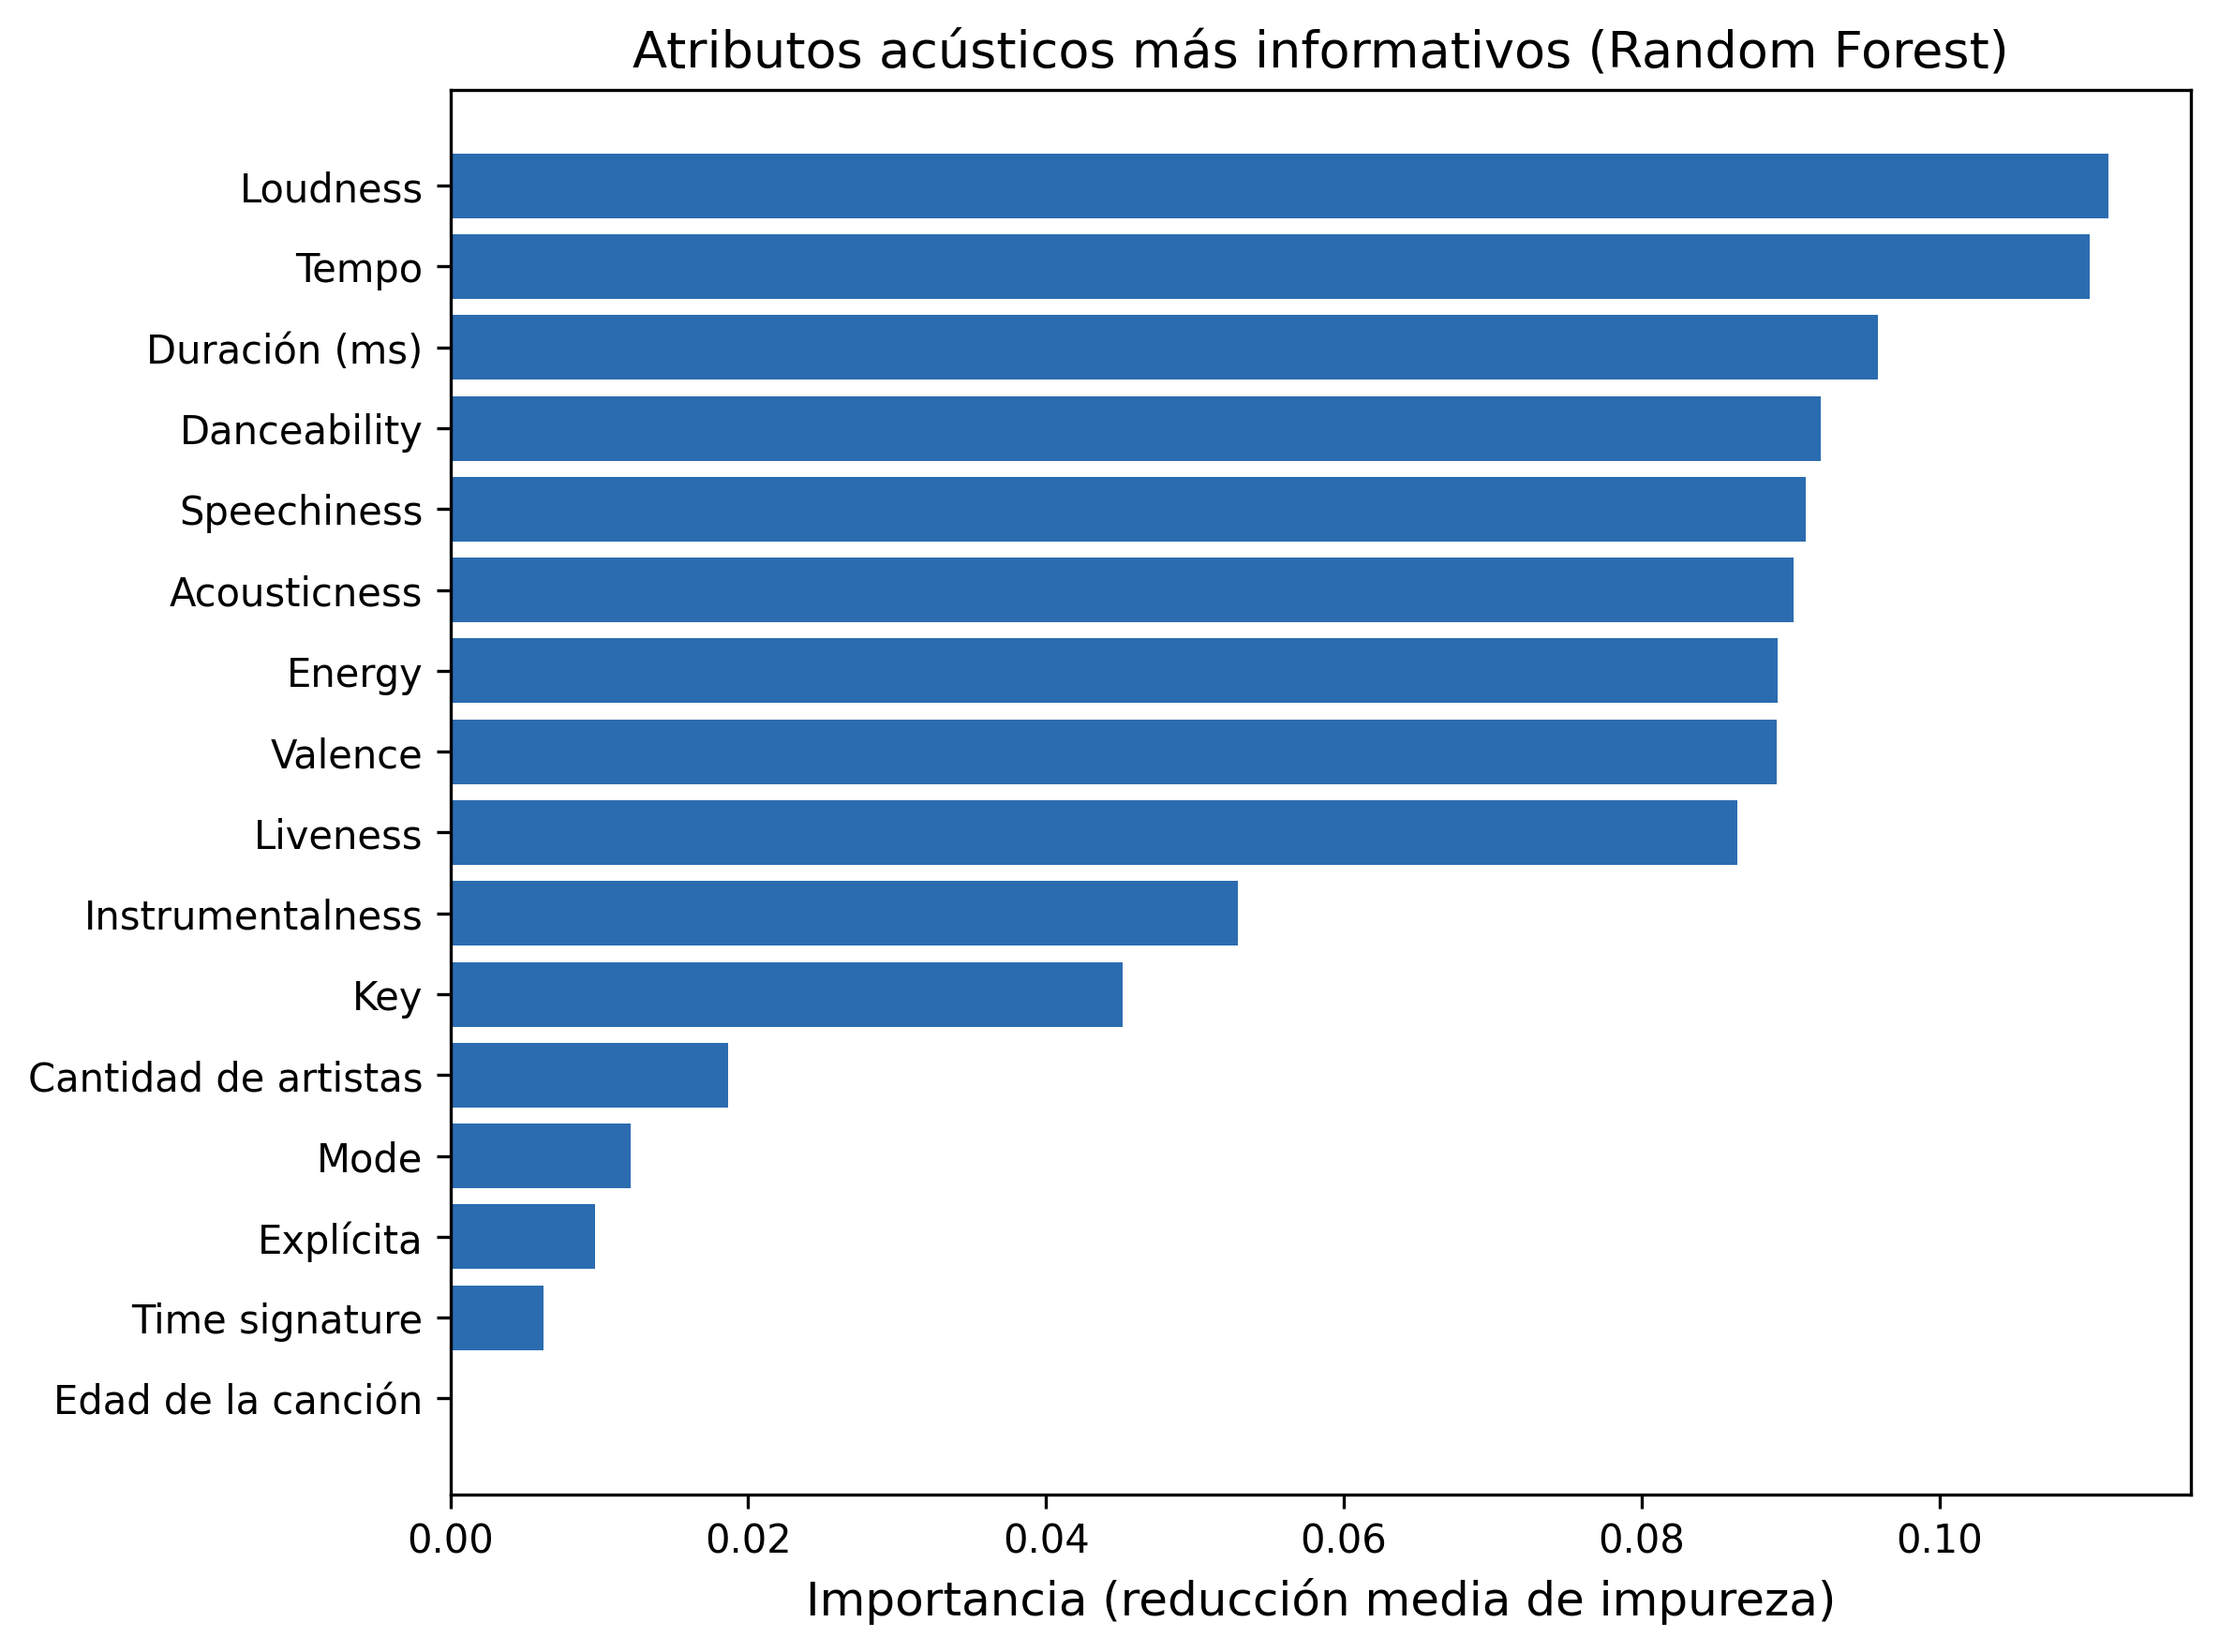
\includegraphics[width=.8\textwidth]{importancia-variables.png}
  \caption{Importancia relativa de los atributos en el Random Forest. Aun los
           más informativos aportan poco en términos absolutos.}
  \label{fig:importancia}
\end{figure}

\subsection{Robustez}

Cabe preguntarse si el pobre desempeño de los atributos acústicos se debe a
lo exigente de la definición de súper hit. La Tabla~\ref{tab:robustez} y la
Figura~\ref{fig:robustez} reestiman el modelo moviendo el umbral de
popularidad desde 30 puntos ---donde un tercio de las canciones califica como
hit--- hasta 80. Para aislar el efecto del umbral, este ejercicio mantiene
fijos los hiperparámetros en lugar de volver a elegirlos en cada punto, de modo
que sus valores de AUC no son estrictamente comparables con los de la
Tabla~\ref{tab:resultados}. El AUC permanece prácticamente constante en torno a
0.72 en todo el rango.

\begin{table}[htbp]
\caption{Desempeño del Random Forest sobre atributos acústicos según el umbral de popularidad usado para definir un hit. La última columna es la proporción de aciertos de una regla que nunca predice un hit.}
\label{tab:robustez}
\begin{tabular}{rrrr}
\toprule
Umbral & Positivos (\%) & AUC & Aciertos triviales \\
\midrule
30 & 34.097 & 0.707 & 0.659 \\
40 & 19.645 & 0.718 & 0.804 \\
52 & 8.530 & 0.724 & 0.915 \\
60 & 3.851 & 0.736 & 0.961 \\
70 & 1.027 & 0.725 & 0.990 \\
80 & 0.201 & 0.681 & 0.998 \\
\bottomrule
\end{tabular}
\end{table}


\begin{figure}[htbp]
  \centering
  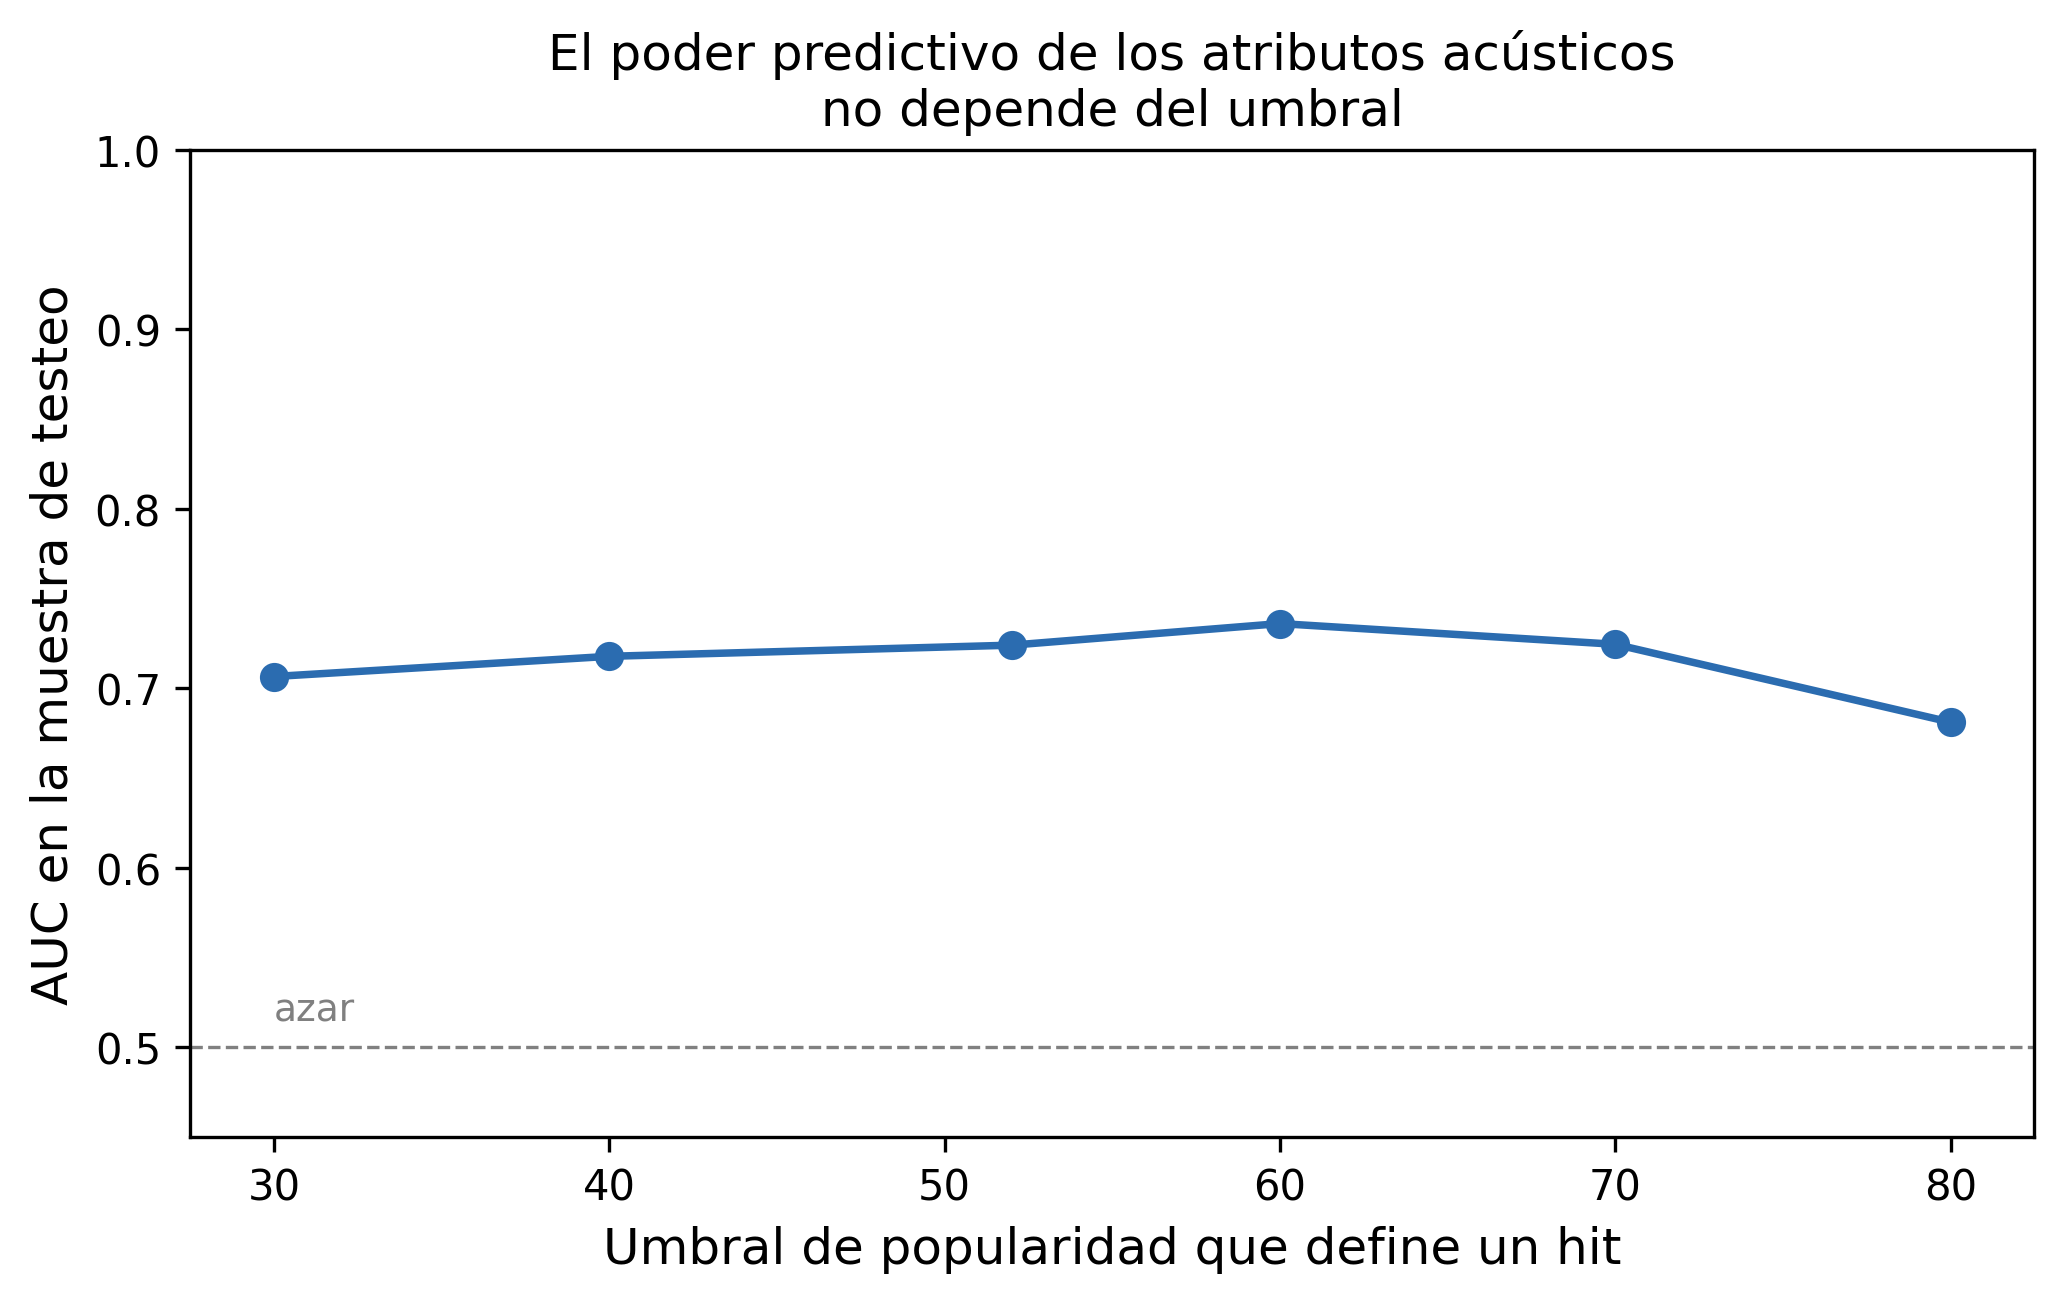
\includegraphics[width=.68\textwidth]{robustez-umbral.png}
  \caption{AUC del Random Forest sobre atributos acústicos según el umbral de
           popularidad que define un hit.}
  \label{fig:robustez}
\end{figure}

La conclusión no es entonces un artefacto del desbalance de clases: los
atributos acústicos informan poco sobre la popularidad en cualquier punto de
la distribución.

\section{Discusión}

\subsection{Relación con la literatura}

Nuestro resultado para los atributos acústicos es sustancialmente más
pesimista que el de los trabajos revisados, que reportan desempeños del orden
del 83\% al 89\% \citep{pareek2022,dimolitsas2023}. Hay al menos tres
explicaciones posibles, no mutuamente excluyentes.

La primera es la métrica. Varios de estos trabajos informan proporción de
aciertos sobre muestras desbalanceadas sin contrastarla contra la tasa base.
Con un 8\% de casos positivos, una regla que nunca predice un hit ya alcanza
el 92\% de aciertos, de modo que un 89\% informado de esa manera no
constituye evidencia de capacidad predictiva. La última columna de la
Tabla~\ref{tab:robustez} hace explícito ese punto de comparación.

La segunda es el conjunto de atributos. Varios trabajos incorporan el género
musical, el artista o métricas sociales externas a la plataforma. Son
predictores razonables de popularidad, pero no son atributos acústicos: se
acercan más a información de trayectoria que a cualidades sonoras de la
canción.

La tercera es la definición de la variable dependiente. Nuestro objeto es el
éxito extremo. Distinguir una canción muy popular de una de popularidad media
es una tarea distinta, y más fácil, que identificar al 1\% superior.

\subsection{Interpretación}

El patrón que surge de los datos tiene una lectura natural. El éxito extremo
es fuertemente persistente: saber que una canción estaba en el extremo
superior el año pasado basta para anticipar que seguirá allí. Pero esa
persistencia no se explica por lo que la canción \textit{es} en términos
sonoros. Es consistente con mecanismos acumulativos ---influencia social,
inclusión en \textit{playlists}, sistemas de recomendación que amplifican lo
que ya es popular--- más que con un conjunto de cualidades intrínsecas que
hagan exitosa a una canción. \citet{salganik2006} documentan
experimentalmente esta clase de dinámica en mercados culturales: cuando los
participantes observan las elecciones de otros, el éxito se vuelve a la vez
más desigual y menos predecible a partir de la calidad intrínseca.

Para quien quisiera usar estos resultados, la implicancia es incómoda: no
parece haber una receta sonora del súper hit. Las variables que sí predicen
son las que describen la posición que la canción ya ocupa.

\subsection{Limitaciones}

Hay cuatro que conviene explicitar.

\textbf{El horizonte es corto.} Observamos 2018 y 2019. Un año de distancia
hace que la persistencia de la popularidad sea casi mecánica, y el ejercicio
dice poco sobre cuán predecible es el éxito de una canción nueva, que es la
pregunta de interés para quien está por lanzarla.

\textbf{La variable dependiente es opaca.} Spotify no documenta cómo se
construye el \textit{popularity score}. Se sabe que combina reproducciones
recientes con recencia, pero su definición exacta es privada, de modo que no
puede descartarse que incorpore componentes que generen persistencia por
construcción.

\textbf{No hay identificación causal.} Todo lo reportado es predictivo. Nada
permite afirmar que modificar un atributo acústico cambiaría la probabilidad
de éxito.

\textbf{El panel sobrevive.} Al quedarnos con las canciones presentes en
ambos años excluimos las que desaparecieron de la plataforma, que
probablemente sean las menos populares. Esto puede comprimir la parte baja de
la distribución.

\section{Conclusión}

Comparamos dos maneras de identificar a las canciones del 1\% más popular de
Spotify sobre un panel de \nPanel{} canciones observadas en 2018 y 2019. Una
ley de potencia ajustada por máxima verosimilitud sobre la popularidad del
año anterior las identifica casi perfectamente; un Random Forest que solo
observa atributos acústicos ordena mejor que el azar pero recupera una fracción
mínima de los súper hits, y el resultado se mantiene en cualquier umbral de
popularidad. Cuando se le agrega la
popularidad pasada, el mismo algoritmo alcanza el desempeño de la ley de
potencia, lo que confirma que la limitación está en la información disponible
y no en el método.

La respuesta a la pregunta del título es entonces doble. Un súper hit se
predice muy bien, pero a partir de su trayectoria, no de su sonido. En un
mercado donde la atención se concentra de manera tan desigual, lo que mejor
anticipa el éxito futuro es el éxito pasado.

\appendix
\section{Correcciones respecto de la versión original}

Esta versión del análisis corrige tres problemas de la implementación
original que afectaban los resultados. Se documentan por transparencia, ya
que modifican las conclusiones del trabajo.

\paragraph{Circularidad.} El modelo de ley de potencia calculaba la
probabilidad a partir de \texttt{popularity\_\allowbreak 2019}, que es la misma variable
con la que se define la etiqueta de súper hit. El modelo predecía la variable
usando la variable misma, de modo que una implementación correcta de esa
especificación habría dado un AUC de exactamente uno por construcción. En
esta versión la ley de potencia se evalúa sobre \texttt{popularity\_2018}.

\paragraph{Fórmula.} La implementación original usaba
$(x/x_{99})^{-(\alpha+1)}$, con el exponente equivocado y el percentil 99 en
lugar de $x_{\min}$. Esa expresión es decreciente en la popularidad ---a
canción más popular le asignaba menor probabilidad de ser un hit--- y toma
valores mayores que uno, lo que es imposible para una probabilidad. La
expresión correcta es la ecuación~\eqref{eq:supervivencia}.

\paragraph{Umbral de decisión.} Clasificar como positivo todo caso con
probabilidad mayor a $0.5$ no funciona con una tasa base del 1\%: casi ningún
caso supera ese valor. Esta versión calibra el umbral de cada modelo a la
tasa base.

Adicionalmente, la búsqueda de hiperparámetros original optimizaba la
proporción de aciertos, que con un 1\% de positivos no discrimina entre
candidatos; aquí se optimiza el AUC. La validación cruzada usaba pliegues sin
estratificar, que con una clase positiva tan chica puede dejar pliegues con muy
pocos positivos; aquí se estratifica. Los filtros de limpieza que comparaban
una fecha contra el entero cero ---una comparación que nunca es verdadera, de
modo que no eliminaban ninguna observación--- se reemplazaron por una
verificación de valores faltantes.

\bibliography{referencias}

\end{document}
